\section{Experiments}
\label{sec:experiments}
We distinguish three evidence blocks: a completed nine-task initialization/objective study, a paused comparison with recent one-step methods, and a completed two-object grasp pilot. None is an original-author-budget RFM reproduction. All numerical claims below use completed runs; interrupted checkpoints appear only in validation diagnostics.

\subsection{Data and Metrics}
Four Earth-event datasets lie on $\mathbb S^2$ (Volcano, Earthquake, Flood, Fire); four protein-angle datasets lie on $\mathbb T^2$ (General, Glycine, Proline, Pre-Pro); RNA uses $\mathbb T^7$. Data follow the RFM pipeline and share a fixed 80/10/10 row split. The local RNA preprocessing has 9,473 rows. These historically inspected splits do not test unseen proteins, temporal forecasting, or independent source groups.

For these nine tasks the primary score is the biased squared MMD V-statistic with $k(x,y)=\exp(-\|e(x)-e(y)\|_2^2/h^2)$, using the identity sphere embedding or circular torus embedding. The bandwidth is fixed from training data. Up to 1,024 held-out points are shared across models; generated batches have the same size. We average three draws within each training seed and report mean and sample SD over seeds 0, 1, 2. The finite-sample biased score need not vanish under the correct law. Intrinsic nearest-neighbor, coverage, 1-NNA, and constraint metrics complement MMD. Exact NLL is unavailable for these implicit generators; sample scores do not reproduce published likelihood tables.

\subsection{Initialization and Objective Controls}
The earlier controlled study uses batch 256, width-128 networks, and AdamW learning rate $2\times10^{-4}$ with no weight decay. Midpoint models take 2,000 outer iterations, each with one critic and one generator update. The smaller controlled RFM runs for 2,000 or 10,000 updates and samples with 128 field calls. These are iteration comparisons, not matched optimizer work or FLOPs. No validation/test checkpoint selection is used in this block.

\begin{table*}[t]
\caption{\textbf{Controlled real-data sample quality.} Biased $\widehat{\mathrm{MMD}}^2\times10^3$ (lower is better), mean $\pm$ sample SD over three training seeds, after averaging three draws per seed. Mixture initialization uses training data only. RFM uses 128 field calls at inference. Budgets are updates/outer iterations, not equal FLOPs; the smaller controlled RFM is not the original author-budget model.}
\label{tab:main}
\centering\small
\begin{tabular}{@{}lrrrrr@{}}
\toprule
Dataset & Test $n$ & Mixture init. & R-MGM mixture (ours) & RFM & RFM (longer) \\
 & & 0 updates & 2,000 iterations & 2,000 updates & 10,000 updates \\
\midrule
Volcano & 82 & $16.20\,\pm\,5.24$ & $13.91\,\pm\,4.89$ & $15.04\,\pm\,1.07$ & $12.86\,\pm\,0.31$ \\
Earthquake & 612 & $1.73\,\pm\,0.65$ & $1.76\,\pm\,0.61$ & $6.17\,\pm\,0.38$ & $3.83\,\pm\,0.32$ \\
Flood & 487 & $1.68\,\pm\,0.51$ & $1.61\,\pm\,0.12$ & $4.04\,\pm\,0.31$ & $2.26\,\pm\,0.39$ \\
Fire & 1024 & $0.73\,\pm\,0.59$ & $1.01\,\pm\,0.58$ & $4.06\,\pm\,0.52$ & $0.91\,\pm\,0.13$ \\
General & 1024 & $0.61\,\pm\,0.06$ & $33.75\,\pm\,3.94$ & $40.69\,\pm\,0.77$ & $23.25\,\pm\,2.20$ \\
Glycine & 1024 & $0.90\,\pm\,0.32$ & $14.29\,\pm\,2.46$ & $18.58\,\pm\,0.88$ & $6.73\,\pm\,0.43$ \\
Proline & 763 & $0.89\,\pm\,0.53$ & $88.86\,\pm\,3.13$ & $94.25\,\pm\,2.35$ & $20.97\,\pm\,1.93$ \\
Pre-Pro & 691 & $1.42\,\pm\,0.35$ & $16.84\,\pm\,15.62$ & $36.64\,\pm\,1.32$ & $17.33\,\pm\,2.21$ \\
RNA (7D) & 947 & $1.52\,\pm\,0.10$ & $2.37\,\pm\,0.20$ & $205.44\,\pm\,1.84$ & $101.07\,\pm\,4.20$ \\
\bottomrule
\end{tabular}
\end{table*}

Table~\ref{tab:main} reports fixed-checkpoint outcomes. Across the 9 fully evaluated tasks, midpoint-trained mixtures have lower mean MMD than their initialization on 2, the 2,000-update flow on 9, and the longer 10,000-update flow on 4. These are descriptive counts, not significance tests or a ranking against author-budget models. Training worsens the mean initialization score on 7 tasks at these settings. The initialization column attributes fit present before training to the restricted mixture model. The degradations expose failures of the implemented finite-critic training procedure, but do not isolate a unique cause or support universal improvement. Figure~\ref{fig:controlled} shows fixed-seed sample visualizations; full-dimensional numerical evaluation is retained for RNA. The matched MMD-trained MLP has lower mean MMD than the midpoint-trained MLP on 3 of 3 representative tasks (Table~\ref{tab:ablation}); these runs do not establish an advantage of the midpoint objective over this direct loss. It also has lower mean nearest-neighbor distance on 3 and higher coverage on 3 of these tasks (supplemental Table~\ref{tab:mlp-metrics}), without implying a universal objective ranking.

\begin{table}[t]
\caption{\textbf{Initialization and objective controls.} Biased MMD$^2\times10^3$, mean $\pm$ SD across three training seeds. All trained rows use 2,000 iterations/updates. MLP rows share architecture and output constraints; mixture rows have a different restricted parameterization.}
\label{tab:ablation}
\centering\small
\setlength{\tabcolsep}{4pt}
\begin{tabular}{@{}lrrr@{}}
\toprule
Method & Fire & General & RNA \\
\midrule
Init. GMM & $0.7\,\pm\,0.6$ & $0.6\,\pm\,0.1$ & $1.5\,\pm\,0.1$ \\
R-MGM GMM & $1.0\,\pm\,0.6$ & $33.8\,\pm\,3.9$ & $2.4\,\pm\,0.2$ \\
R-MGM MLP & $21.4\,\pm\,16.4$ & $60.7\,\pm\,10.8$ & $283.0\,\pm\,119.0$ \\
MMD MLP & $2.2\,\pm\,0.7$ & $31.1\,\pm\,0.8$ & $8.5\,\pm\,0.7$ \\
RFM (1) & $27.5\,\pm\,2.3$ & $61.0\,\pm\,1.5$ & $343.6\,\pm\,4.6$ \\
RFM (128) & $4.1\,\pm\,0.5$ & $40.7\,\pm\,0.8$ & $205.4\,\pm\,1.8$ \\
\bottomrule
\end{tabular}
\end{table}




The mixture starts from train-fitted centers, scales, and weights; only centers and scales receive pathwise midpoint gradients. Hard component boundaries leave weights fixed. Matched random-MLP midpoint and direct-MMD controls isolate objective choice on three tasks. The direct-MMD control is not KGDM or RW-Flow. These results expose substantial optimization failures rather than a general efficacy claim. Post hoc, single-seed validation diagnostics examine periodic features, critic warmup, extra critic steps, and a true-velocity randomized torus path (\cref{app:stability}); they do not alter this table.

\subsection{Recent One-Step Comparisons: Completed Cells}
\label{sec:recent}
We implement RW-Flow-C \citep{nurgulan2026rwflow}, KGDM \citep{estebancasadevall2026kgdm}, and the RMF-MT variant of \citet{zhong2026rmf}. This is the latter MeanFlow construction, not the distinct method of \citet{woo2026rmf}. Midpoint, RW-Flow-C, and KGDM share an unfitted, uniform-prior point generator with width 128, three affine layers, and 16 latent dimensions. RMF retains its source-derived two-time network, with a different parameter count. Every sampler uses one neural evaluation. Method-source fidelity and adaptations are detailed in \cref{app:recent-protocol}.

Configurations are selected on representative validation tasks and frozen before final tests. Completed jobs use 50,000 generator/field updates, batch 256, and validation-selected checkpoints, including initialization. MGM additionally uses 500 critic warmup updates and five or ten critic updates per generator update. Critic refinement, tuning grids, model parameters, and compute are not matched.

\begin{table*}[t]
\centering\small
\caption{\textbf{Completed modern one-step comparisons.} Test $\widehat{\mathrm{MMD}}_V^2\times10^3$, mean $\pm$ training-seed SD (three seeds); lower is better. Each available cell completed 50,000 generator/field updates and uses a validation-selected checkpoint. All samplers use one network evaluation. The paused 108-job plan has only 18 completed jobs; n/a means unavailable, not a performance score. These are small-network adaptations, not original-author benchmark reproductions.}
\label{tab:recent}
\begin{tabular}{@{}llrrrr@{}}
\toprule
Dataset & Test $n$ & R-MGM (ours) & RW-Flow-C & KGDM & RMF-MT \\
\midrule
Volcano & 82 & $13.135\,\pm\,1.555$ & $12.537\,\pm\,0.277$ & $13.900\,\pm\,1.694$ & $11.957\,\pm\,0.275$ \\
Earthquake & 612 & n/a & n/a & $2.132\,\pm\,0.115$ & $2.814\,\pm\,0.694$ \\
\bottomrule
\end{tabular}
\end{table*}

\Cref{tab:recent} reports the completed cells of the nine-task, four-method, three-seed plan: 18 of 108 jobs at this snapshot. Only Volcano supports a completed four-method comparison. Its smallest observed mean is RMF-MT's; MGM does not outperform it, and no significance claim is made. Earthquake has only KGDM and RMF-MT completed across all seeds; its two interrupted MGM runs have no test results. Remaining tasks are unavailable, not negative scores. \Cref{fig:recent-volcano} shows fixed seed-0 samples; recorded validation curves appear in \cref{fig:recent-curves}. A 50,000-update cap does not certify convergence. Training shared one GPU between at most two workers; isolated latency profiling was not run, so this block supplies no inference-speed or training-efficiency ranking.

\begin{figure*}[t]
\centering
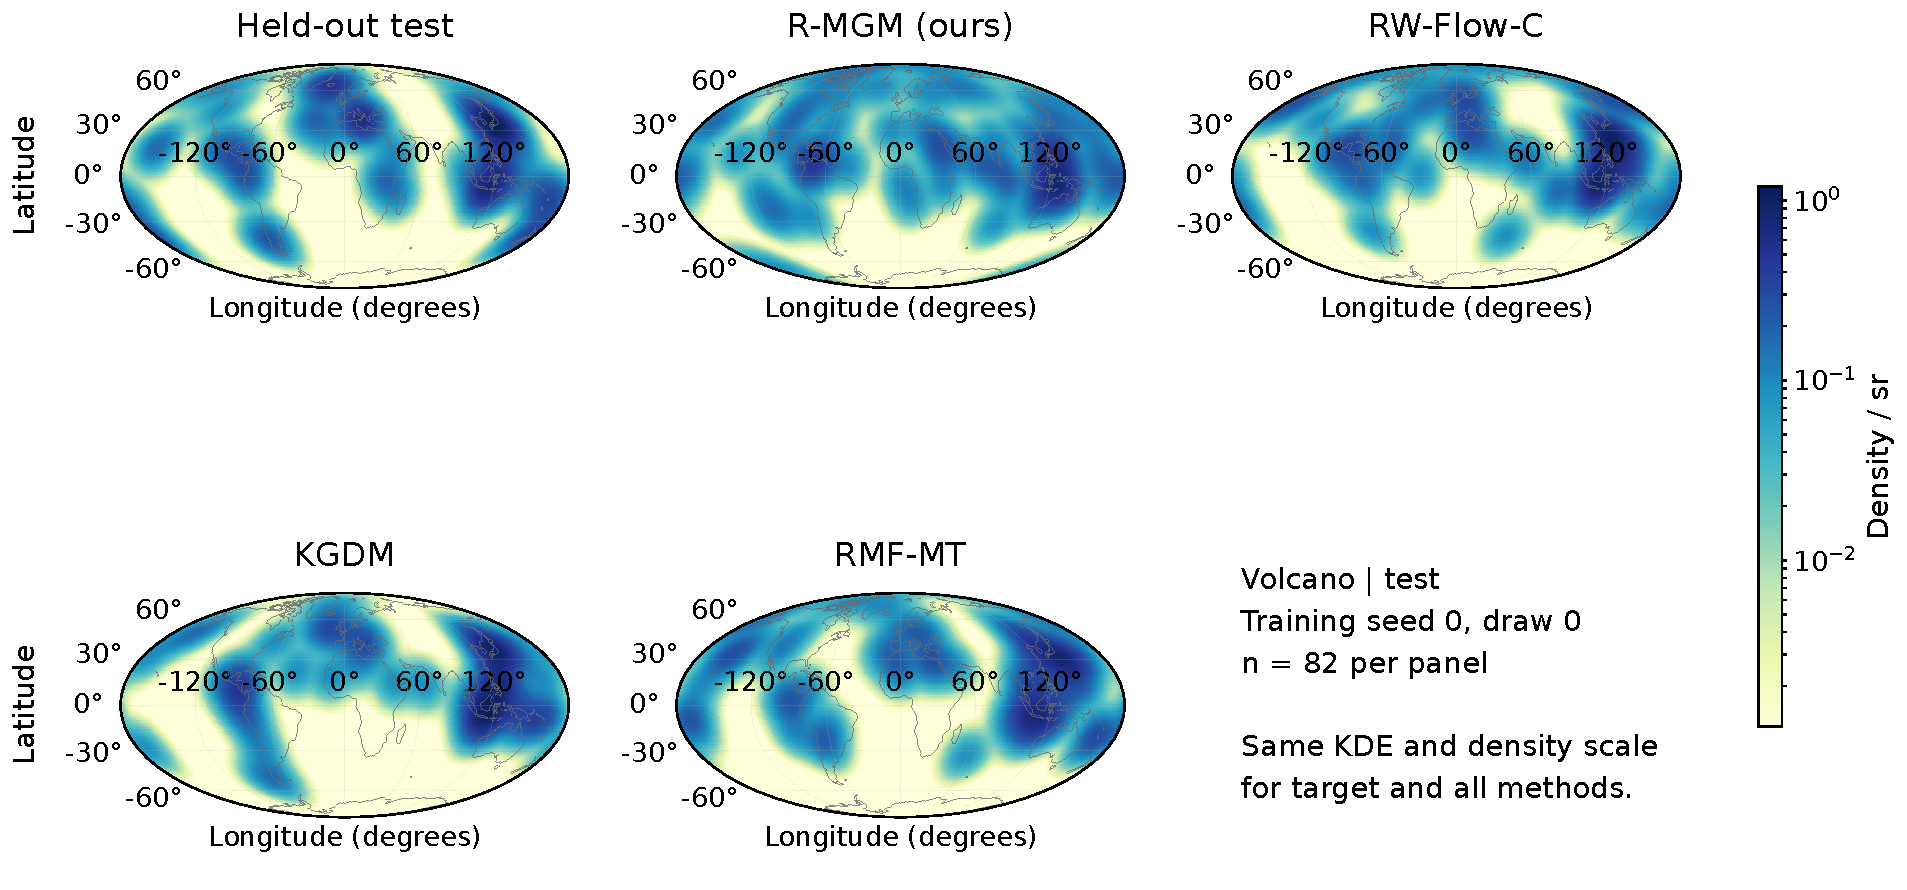
\includegraphics[width=.94\textwidth]{figures/recent_volcano.pdf}
\caption{\textbf{Completed one-step comparison on Volcano.} Fixed test target and training seed 0, generated draw 0; $n=82$ per panel. Checkpoints are validation-selected after each run completed 50,000 updates. All panels use the same spherical KDE and logarithmic density scale. These are sample densities, not likelihoods or additional independent training seeds. Quantitative means use all three seeds in \cref{tab:recent}.}
\label{fig:recent-volcano}
\end{figure*}

\subsection{SE(3) Grasp Proposals}
\label{sec:grasp}
We use the two public, matched Mug/Table HDF5 and mesh examples from ACRONYM \citep{eppner2021acronym}. Positive source poses are split 80/10/10 within each known object; this is not full ACRONYM or unseen-object transfer. The product $SO(3)\times\R^3$ geometry constrains rotations and normalizes translation from mesh bounds. Each of MGM, local RFM, and a source-loss RMF-MT adaptation completes 10,000 generator/field updates for three seeds. No validation/test tuning or checkpoint selection is used; MGM adds 100 warmup and 50,000 critic updates per seed. RFM uses 50 or 100 inference evaluations, while MGM and RMF-MT use one. Architecture and path adaptations preclude an original-author grasp reproduction.

\begin{table*}[t]
\centering\small
\caption{\textbf{Completed two-object SE(3) pilot.} Equal object means are formed within each training seed, then mean $\pm$ sample SD over three seeds. Every model trains for 10,000 generator/field updates. Pose MMD is an \emph{unbiased product-kernel} statistic, distinct from \cref{tab:main,tab:recent}. The thin-gripper static proxy is not physical success; full-Franka collision tests a different geometry. Reference poses have 92\%/100\% static-proxy passes on Mug/Table and 0\% full collisions. Lower pose MMD and collision, but higher proxy fraction, are better.}
\label{tab:grasp}
\begin{tabular}{@{}lrrrr@{}}
\toprule
Method & NFE & Pose MMD$^2\times10^3$ & Static proxy (\%) & Full collision (\%) \\
\midrule
R-MGM (ours) & 1 & $4.265\,\pm\,1.591$ & $24.67\,\pm\,1.76$ & $71.00\,\pm\,5.22$ \\
RMF-MT adaptation & 1 & $12.096\,\pm\,1.458$ & $10.83\,\pm\,2.47$ & $34.17\,\pm\,0.29$ \\
RFM & 50 & $0.530\,\pm\,0.099$ & $32.17\,\pm\,3.51$ & $67.00\,\pm\,2.50$ \\
RFM & 100 & $0.515\,\pm\,0.119$ & $32.00\,\pm\,3.28$ & $66.67\,\pm\,2.25$ \\
\bottomrule
\end{tabular}
\end{table*}

\Cref{tab:grasp} averages the two object scores within each seed before computing seed SD. Pose MMD is an unbiased chordal-product-kernel statistic and is not numerically comparable with the sphere/torus score. Static geometric checks use 100 unfiltered draws per object; distribution metrics use 512 generated poses. MGM has lower pose MMD and higher thin-gripper static-proxy fraction than this one-step RMF-MT adaptation, but multi-step RFM is more accurate in pose MMD. MGM's $71.00\%$ mean full-Franka collision rate remains unresolved. Lower collision alone can also reward proposals that miss the object. No finger closure, friction, lifting, scene collision, or reachability is simulated; physical success is unmeasured. \Cref{fig:grasp-current,app:grasp-protocol} give the fixed-sample visualization and protocol.

\subsection{Other Geometries and Numerical Checks}
Float64 endpoint, reversal, and numerical derivative checks on sphere, torus, SPD, and an approximate hyperbolic branch verify implementation conventions, not every floating-point trajectory. Earlier sampling-cost measurements apply only to their recorded architectures and are retained in \cref{app:additional}. On Bunny/Spot targets $k=10,50,100$, historical one-seed, fixed-step-800 runs compare projected mixtures and sphere-map parameterizations. They use the local projected-chord surrogate of \cref{eq:mesh-surrogate}, outside the exact-path theorem; they do not reproduce intrinsic mesh likelihoods. Full figures, controls, and benchmark-coverage limits remain in \cref{app:additional,app:inventory}.
